\section{Method}

\setLayout{mainpoint}

\begin{frame}[noframenumbering, plain]{}
    \frametitle{Method}
\end{frame}

\setLayout{blank}

%---------------------------------------------------------
\begin{frame}{Overview}
    \begin{figure}[!htb]
    \centering
        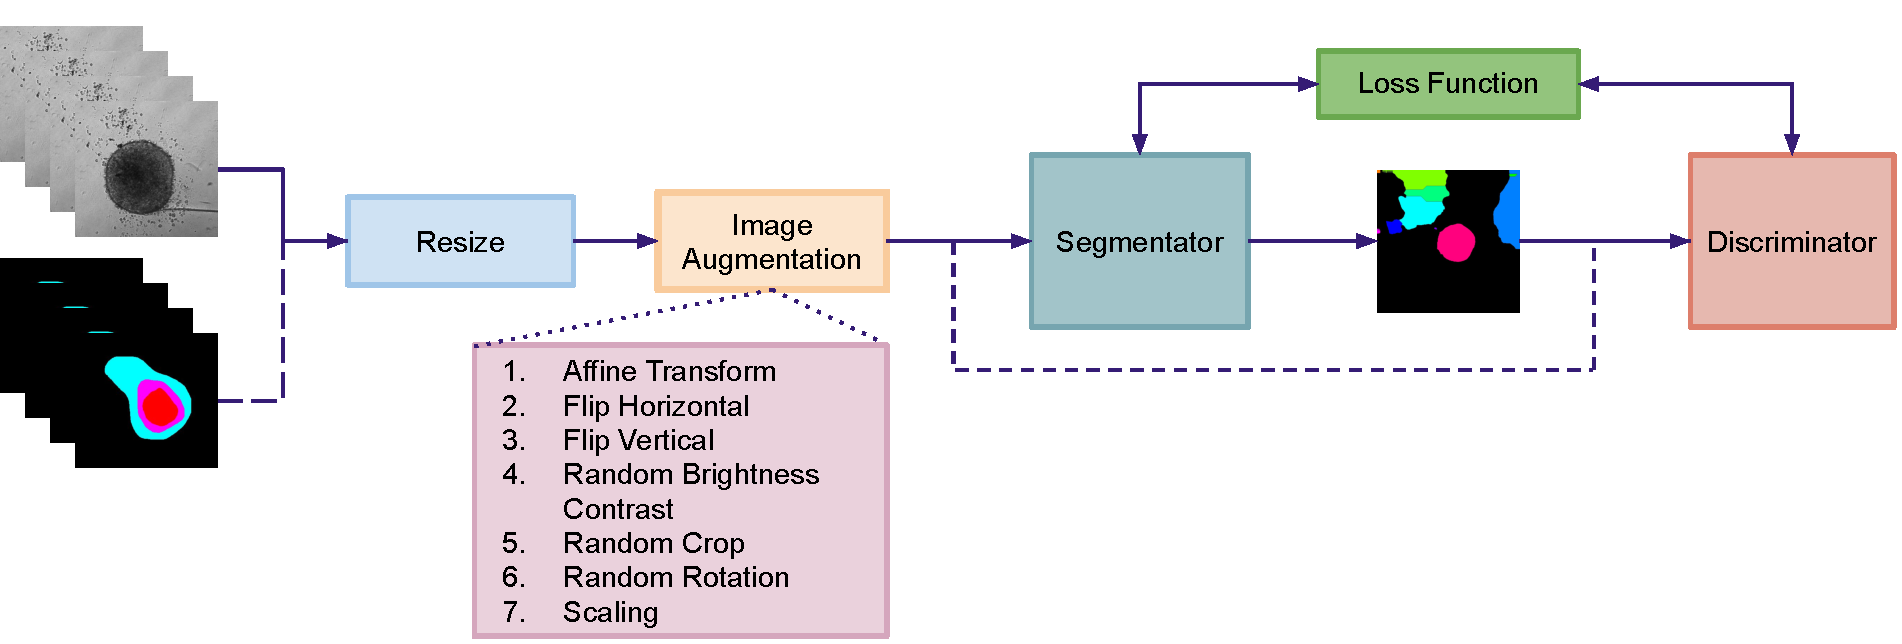
\includegraphics[width=15cm]{figures/method/overview}
        \label{fig:method_overview}
    \end{figure}
\end{frame}

%---------------------------------------------------------
\setLayout{horizontal}

\begin{frame}{Data Augmentation}
    \begin{figure}
        \centering
        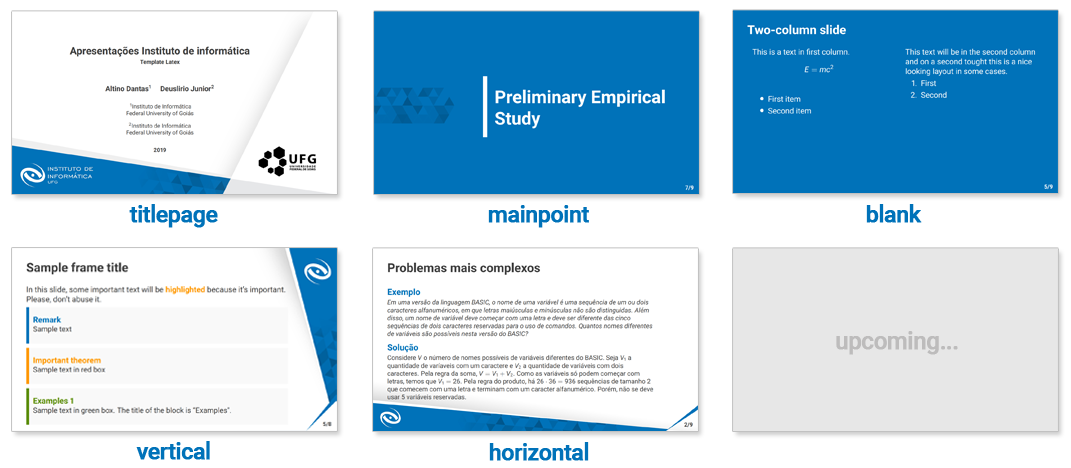
\includegraphics[width=.9\textwidth]{readme/layouts.png}
        \caption{Template's Layouts.}
        \label{fig:data_aug}
    \end{figure}
\end{frame}

%---------------------------------------------------------
\setLayout{blank}

\begin{frame}{Generator Architecture}
    \begin{figure}[!htb]
        \centering
        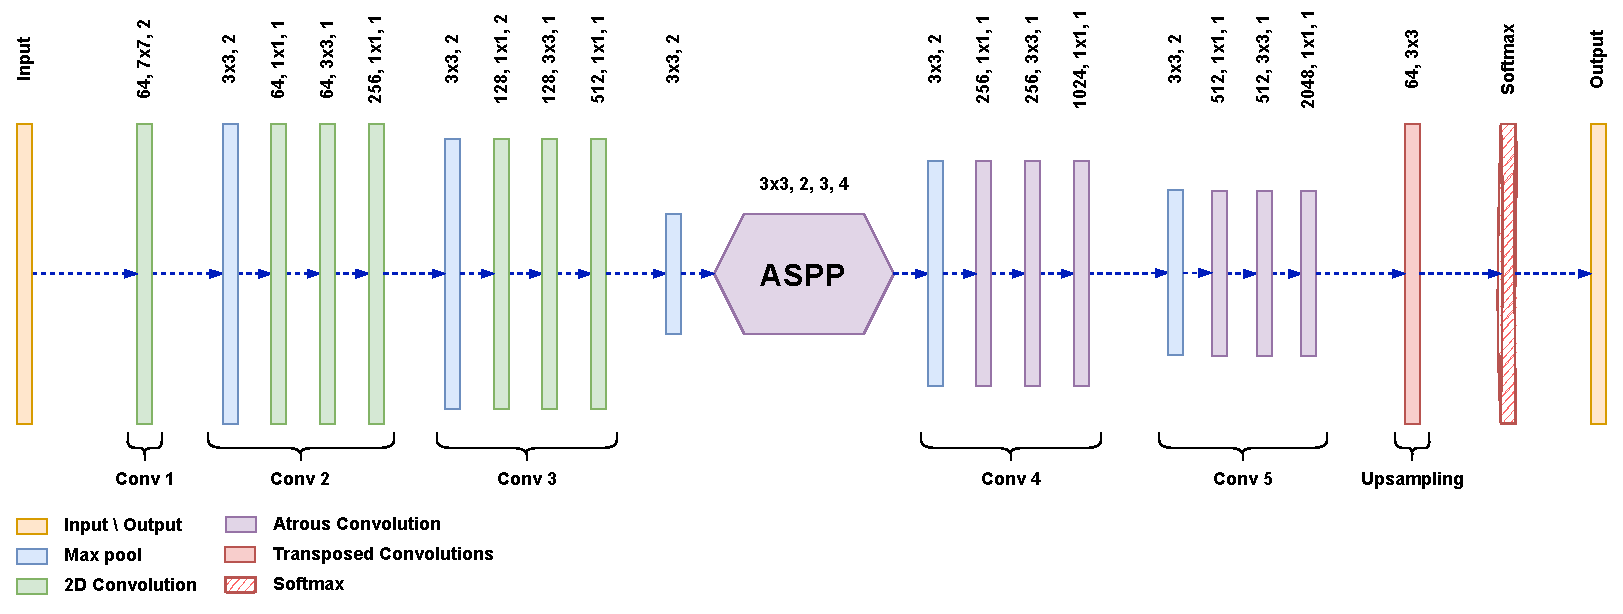
\includegraphics[width=14cm]{figures/method/generator_architecture}
    \end{figure}
\end{frame}

%---------------------------------------------------------

\begin{frame}{Discriminator Architecture}
    \begin{figure}[!htb]
        \centering
        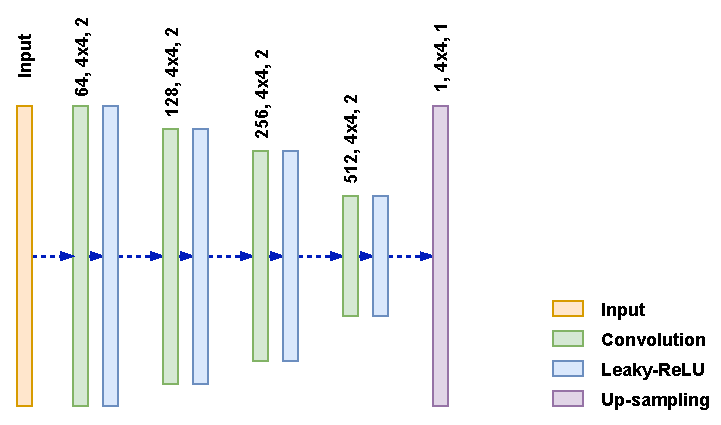
\includegraphics[width=10cm]{figures/method/discriminator_architecture}
    \end{figure}
\end{frame}

%---------------------------------------------------------
\setLayout{vertical}

\begin{frame}{Loss Functions}
    \begin{block}{Generator Loss}
        \begin{equation}
            \mathcal{L}_{semi} = -\sum_{h, w} \sum_{c \in{} C} I(D(G(X_n))^{h, w} > T_{semi})\cdot \gamma_{n}^{(h, w, c)} \log(G(X_n)^{(h, w, c)})
        \end{equation}
    \end{block}
    \begin{block}{Discriminator Loss}
        \begin{equation}
            \mathcal{L}_{D} = -\sum_{h, w}(1-y_n) \log(1-D(G(X_n))^{(h, w)} + y_n \log(D(Y_n)^{(h, w)})
        \end{equation}
    \end{block}
\end{frame}

%---------------------------------------------------------
\begin{frame}{Evaluation Metrics}
    \begin{columns}
        \column{0.5\textwidth}
        \begin{block}{Dice Coefficient}
        \end{block}
        \column{0.5\textwidth}
        \begin{block}{Jaccard Index}
        \end{block}
    \end{columns}
\end{frame}

%---------------------------------------------------------
\begin{frame}{Watershed}
    \begin{figure}
        \centering
        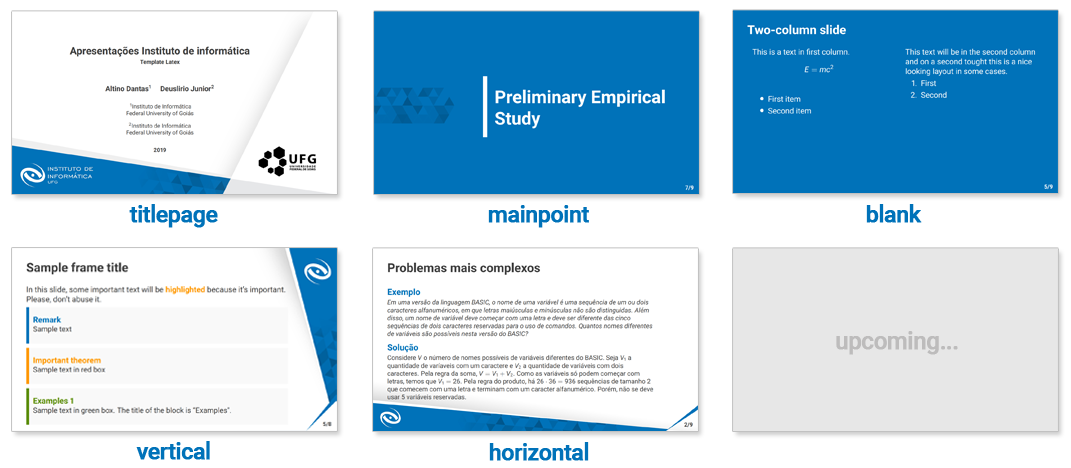
\includegraphics[width=.9\textwidth]{readme/layouts.png}
        \caption{Template's Layouts.}
        \label{fig:watershed}
    \end{figure}
\end{frame}
